% This is samplepaper.tex, a sample chapter demonstrating the
% LLNCS macro package for Springer Computer Science proceedings;
% Version 2.20 of 2017/10/04
%
\documentclass[runningheads]{llncs}
%
\usepackage{graphicx}
% Used for displaying a sample figure. If possible, figure files should
% be included in EPS format.
%
% If you use the hyperref package, please uncomment the following line
% to display URLs in blue roman font according to Springer's eBook style:
% \renewcommand\UrlFont{\color{blue}\rmfamily}

\begin{document}
%
\title{ScSpark: Low-Redundancy disk access and High-Performance tool for the Single-Cell RNA sequenceing data processing\thanks{Supported by organization x.}}
%
%\titlerunning{Abbreviated paper title}
% If the paper title is too long for the running head, you can set
% an abbreviated paper title here
%
\author{First Author\inst{1}\orcidID{0000-1111-2222-3333} \and
Second Author\inst{2,3}\orcidID{1111-2222-3333-4444} \and
Third Author\inst{3}\orcidID{2222--3333-4444-5555}}
%
\authorrunning{F. Author et al.}
% First names are abbreviated in the running head.
% If there are more than two authors, 'et al.' is used.
%
\institute{Princeton University, Princeton NJ 08544, USA \and
Springer Heidelberg, Tiergartenstr. 17, 69121 Heidelberg, Germany
\email{lncs@springer.com}\\
\url{http://www.springer.com/gp/computer-science/lncs} \and
ABC Institute, Rupert-Karls-University Heidelberg, Heidelberg, Germany\\
\email{\{abc,lncs\}@uni-heidelberg.de}}
%
\maketitle
%
\begin{abstract}
High-throughput single-cell RNA sequencing
  (scRNA-seq) data processing pipelines use multiple steps to transform raw scRNA-seq data to gene express matrices, including sequence quality control, genome alignment and transcript counting.
With the incresasing of scRNA-seq data volume, traditional tools' speed and file input/output (IO) becomes the bottleneck of performance.
We took advantage of Apache Spark's in-memory computing and scalable trait to develop a new Java-based program called ScSpark.
ScSpark can distribute scRNA-seq data and process tasks in the cluster.
Also it can significantly reduce disk accessing for intermediate results.
We combined Spark and our proposed function to implement sequence quality control and transcript counting.
And we encapsulated STAR's code as shared object and invoked the shared object as our aligner.
In order to avoid unneccessary disk accessing while reading FASTQ file and writing SAM file, we used Java Native Interface (JNI) to deliver FASTQ RDD's data, and then abstract return value to SAM RDD.
We build spark's cluster on Aliyun to test ScSpark.
The experiment results indicates ScSpark more efficient and more scalable than any tradition tools.
\keywords{Intermediate Data \and Fast \and Scalable.}
\end{abstract}

\section{Introduction}
Individual cells are the smallest unit of life, such as tissues and organs.
According to the central dogma of molecular biology, one of the major factors that determines the function of every cell is its transcriptional program.
In the era of precision medicine, scientific experiments to explore the function of each cell have become crucial.
In the past decade, RNA-Seq has been widely used to study gene expression patterns.
However, the analysis accuracy of RNA-seq could only reach the level of the cell population, and the final difference between samples was the average difference of the cell population. 
But from the molecular point of view, human cells are not exactly the same, there are differences between cells.
Single-cell RNA sequencing essentially reveals the transcriptional status at the single cell level, which provides the basis for subsequent bioinformatics analysis~\cite{Papalexi2018SinglecellRS}.

High-throughput single-cell RNA-seq protocols (HTscRNA-seq), which allow us to sequence thousands of cells simultaneously in a single experiment, are the most popular strategies currently for scRNA-seq technology~\cite{Zhang2019ComparativeAO}. Drop-seq~\cite{Macosko2015HighlyPG}, inDrop~\cite{Klein2015DropletBF} and 10X\cite{zheng2017Massivelypd} are the three most widely used HTscRNA-seq protocols.
Among them, 10X is becoming one of the most prevalent platforms.

Two separate barcode, named cell barcode (CB) and unique molecular identifier (UMI) are introduced in HTscRNA-seq~\cite{Rosenberg2018SinglecellPO}~\cite{Cao2017ComprehensiveSC}.

The CB, which assigns different sequences to each cell for transcriptional source retrieval after sequencing, greatly increases the total length of sequence and reduces the cost of scRNA-seq~\cite{Macosko2015HighlyPG}~\cite{Klein2015DropletBF}.

These barcodes allow reads to be demultiplexed after the cells have been assembled for sequencing.~\cite{tian2018scPipe}.
Apart from cell barcodes, UMIs are random oligonucleotide barcodes that are used in HTscRNA-seq experiments~\cite{Kivioja2012Counting}~\cite{camara2017Methods}.
By UMI, the same copy from different molecules and the same copy from the same molecule for PCR amplification could be distinguished. ~\cite{smith2017UMI}.

In the scRNA-seq experiment, the use of multi-level barcodes presented additional challenges for data processing, which was quite different from traditional bulk RNA-seq and low-throughput scRNA-seq experiments.
In recent years, researchers have developed multiple scRNA-seq data processing tools, typically implementing steps including sequence quality control, genome alignment, and transcript counting to convert raw scRNA-seq data into a gene expression matrix for further downstream analysis.
The first step will filter FASTQ readings with low quality CB based on user-defined thresholds.
This step eliminates most of the false CBs, greatly improving the accuracy of the CBs that need to be considered for counting and reducing the number of CBs in further step.
The remaining FASTQ reads will map to genomes using the splice-aware aligner, such as STAR~\cite{dobin2012RNA} or HISAT2~\cite{kim2015hisat}.
Among them, STAR is the most widely used. A number of popular scRNA-seq data processing tools use STAR for this step, such as UMI-Tools, CellRanger, zumis, scPipe, and STARsolo.
Previous baseline studies have shown that STAR is one of the most reliable reference genomic aligner for RNA-Seq analysis~\cite{Baruzzo2017SimulationbasedCB}.
Next, reads are assigned to genes and then generate count tables for UMIs and reads per gene per CB~\cite{swati0zUMIs}.

Nowadays, there are many tools to deal with scRNA-seq, among which the most popular is CellRanger~\cite{zheng2017Massively}, UMI-tools~\cite{Smith2017UMItoolsMS} and STARsolo~\cite{2019STARsolo}. 
UMI-tools~\cite{ref_url1} is an open source tool with an impressively clear process, our ScSpark is based on improvements to this tool.
CellRanger is a highly integrated data process software tailored by 10X Genomics for single-cell RNA sequencing analysis and it performs comparatively well on machine with enough CPU and memory resources in the big data set, but did badly in small data set. CellRanger performs best under large data sets among existing tools~\cite{gao2020Comparison}.
STARsolo~\cite{2019STARsolo} has improved the parallelism of sequence mapping and counting procedures, and achieved good performance on a single machine.
It is a pity that all tradition tools only run on a single machine with slow running speed, and cannot be extended to multiple nodes.

There have been many studies using big data framework like 
                                                           Hadoop~\cite{ref_url2}
                                                                                  and Spark~\cite{ref_url3} to optimize Next-Generation-Sequencing (NGS) Data Processing.
Due to more efficiency in utilizing memory computing, Spark is a better big data computing framework than Hadoop's MapReduce~\cite{dean2008mapreduce}~\cite{zaharia2012resilient}.
SparkBWA~\cite{abuin2016sparkbwa} and GPF~\cite{li2018high} are good frameworks that both improve the efficiency of NGS data processing by Spark.
In the research area of scRNA-seq, Falco~\cite{Yang2016Falco} has tried to use Spark in scRNA-seq upstream data processing, but it has two serious problems.

Firstly, Falco can't deal with CBs and UMIs, so it can't compatible with any HTscRNA-seq protocol.

Secondly, Falco only uses Spark to simply concatenate the aligner software and the feature quantitative software, which does not reduce the amount of disk reads and writes between the two steps.

Falco’s operations have lots of redundancy disk access which causes its insufficient utilization of Spark’s in-memory computation well.

The increase of scRNA-seq data requires more efficient and faster data processing tools. However, the original scRNA-seq data processing tools were designed without considering of the scalability, which could only run on a single computer and could not be extended to a cluster. From UMI-Tools and CellRanger to STARsolo, parallelism and performance has increased; However, due to the limit of a single machine, scalability is limited.

Refer to Falco's idea of using Spark framework to solve the problem of HTscRNA-seq data processing, we make full use of Spark's parallel and in memory compute advantage, totally use Spark's function to implement sequence quality control but not like Falco use tradition pipeline.
And different with Falco, we enhance STAR's file I/O interface, to reduce redundant disk access.
In the end, scSpark has implemented transcript counting by combining Spark function and our algorithm to achieve parallel compute.
The traditional single machine serial processing mode has been unable to meet the demand of computing and storage resources for super-large scale scRNA-seq data.
Our work plans to adopt Spark system architecture propose a set of in memory computing and scalable scRNA-seq data processing tool, which can significantly reduce the processing time.

\section{Method}
\subsection{Overview}
We implemented scSpark based on Spark framework to utilize Spark's advantage.
We run program across the cluster, and default cache data in memory.
With increasing of dataset volume, the time to process intermediate result file occupies a more significant proportion on total time.
And single machine's capacity is not sufficient to adapt the increasing scRNA-seq data volume.
Therefore, reducing the disk access of intermediate result file and improving the upstream data process's scalability is our scSpark's way to improve tradition pipeline.

\subsection{Spark Version Sequence Quality Control}
\begin{figure}
  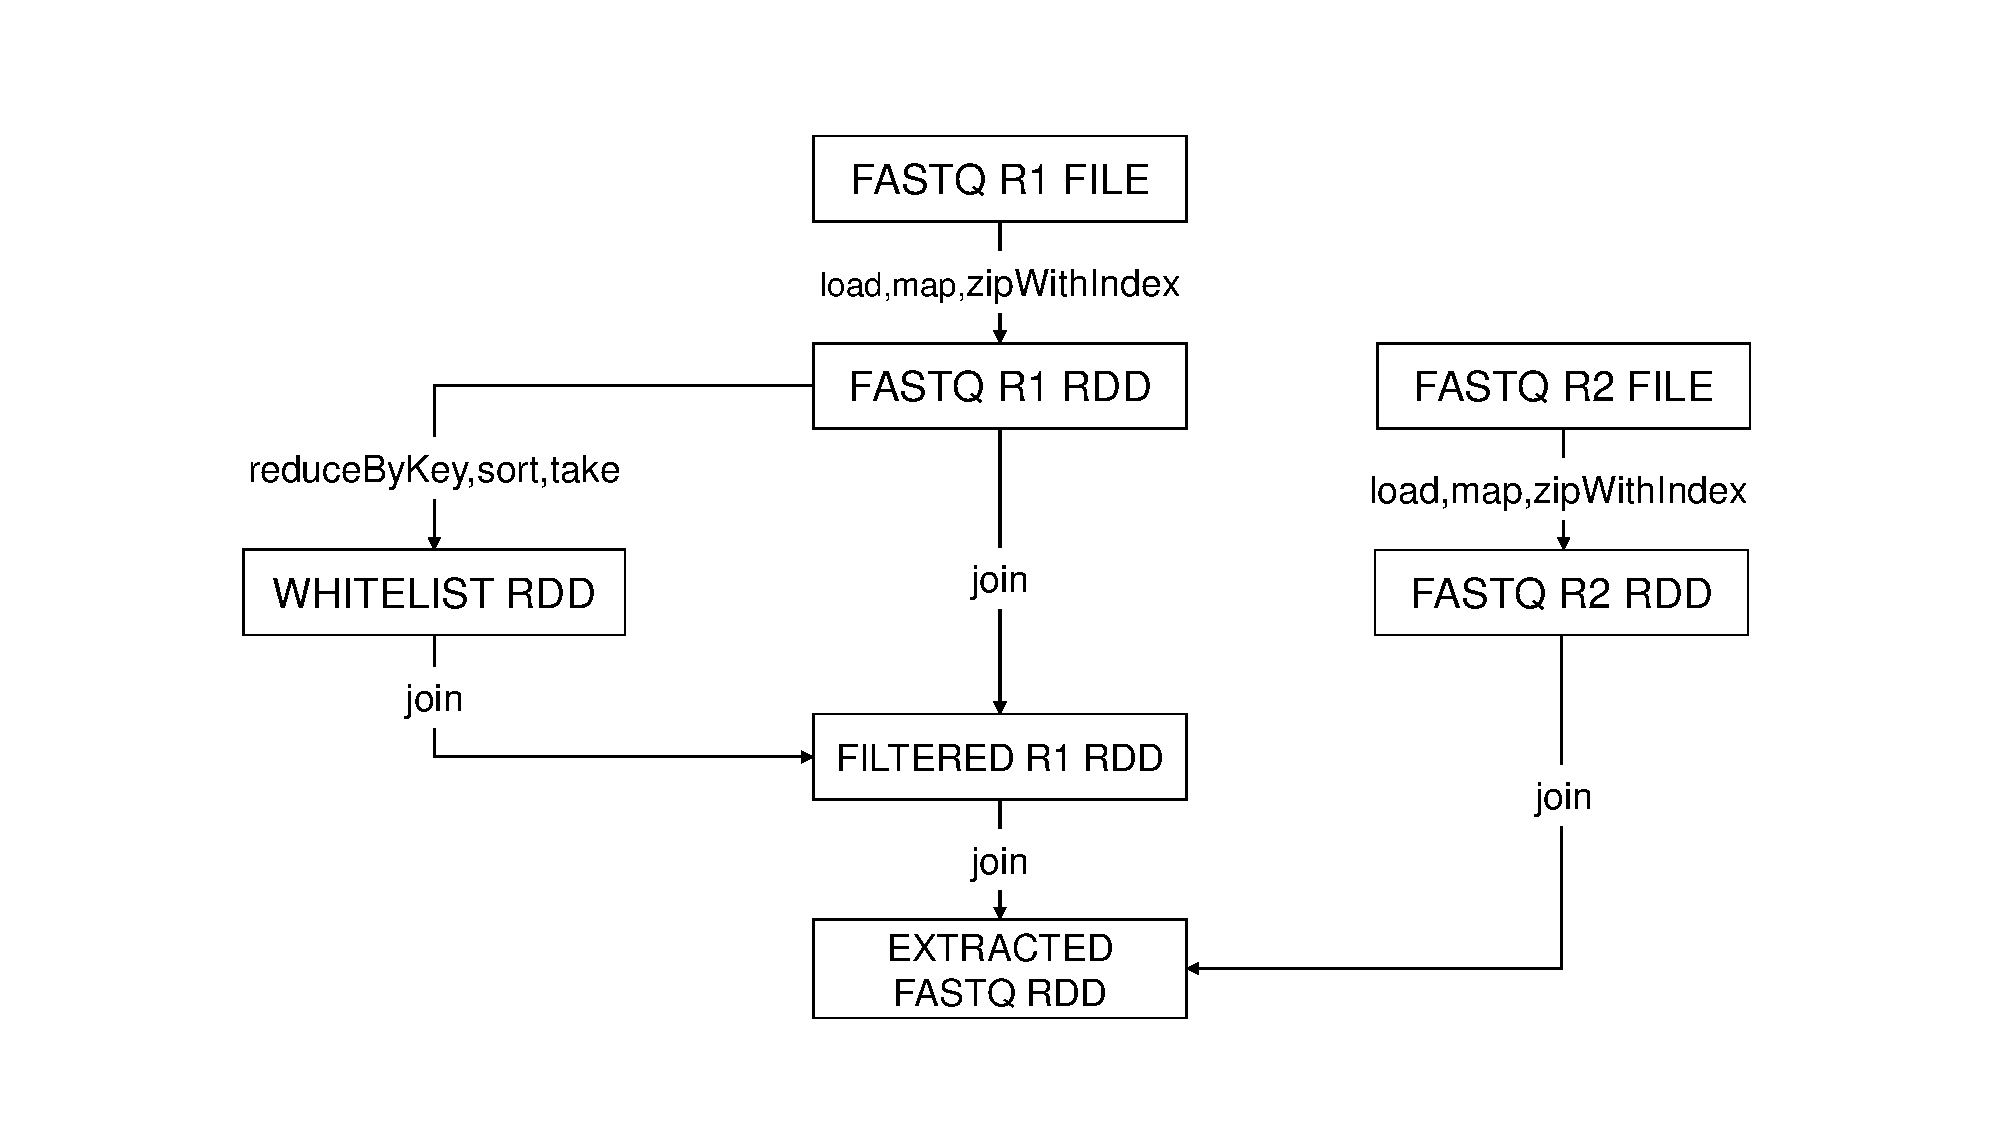
\includegraphics[width=\textwidth]{fig1.pdf}
  \caption{An overview of Spark version Sequence Quality Control.} \label{fig1}
\end{figure}  
Large FASTQ file can load files in each node's memory parallel therefore the loading speed doesn't limit by single node disk access speed.
As shown in Fig~\ref{fig1}, the sequence quality control step typically consists of two main components, generate whitelist which can identity of the true cell barcodes is unknown and then use the whitelist to filter FASTQ R1 and then extract FASTQ R2 according to filtered FASTQ R1's index.

We loaded each file splits of FASTQ R1 to memory, and abstract them as FASTQ R1 RDD.
Then we counted each CB appear times, and selected the most frequent CBs as intermediate result which named whitelist RDD.
By using reduceByKey function, FASTQ R1 RDD can count every barcodes parallel in each splits and sum each split's result in the end.
After that we can use the result to generate whitelist RDD by Spark's sort and take function, both can parallel compute in the cluster.
We can easily get filtered FASTQ R1 RDD, by using the join function to find which read's cell barcode is in the whitelist RDD.
And then we used filter function to extract FASTQ R2 RDD.
The last step in sequence quality control was using join function again to combine filtered FASTQ R1 RDD and FASTQ R2 RDD with same index.
\subsection{Eleminate redundancy disk access in Aligner step}
\begin{figure}
  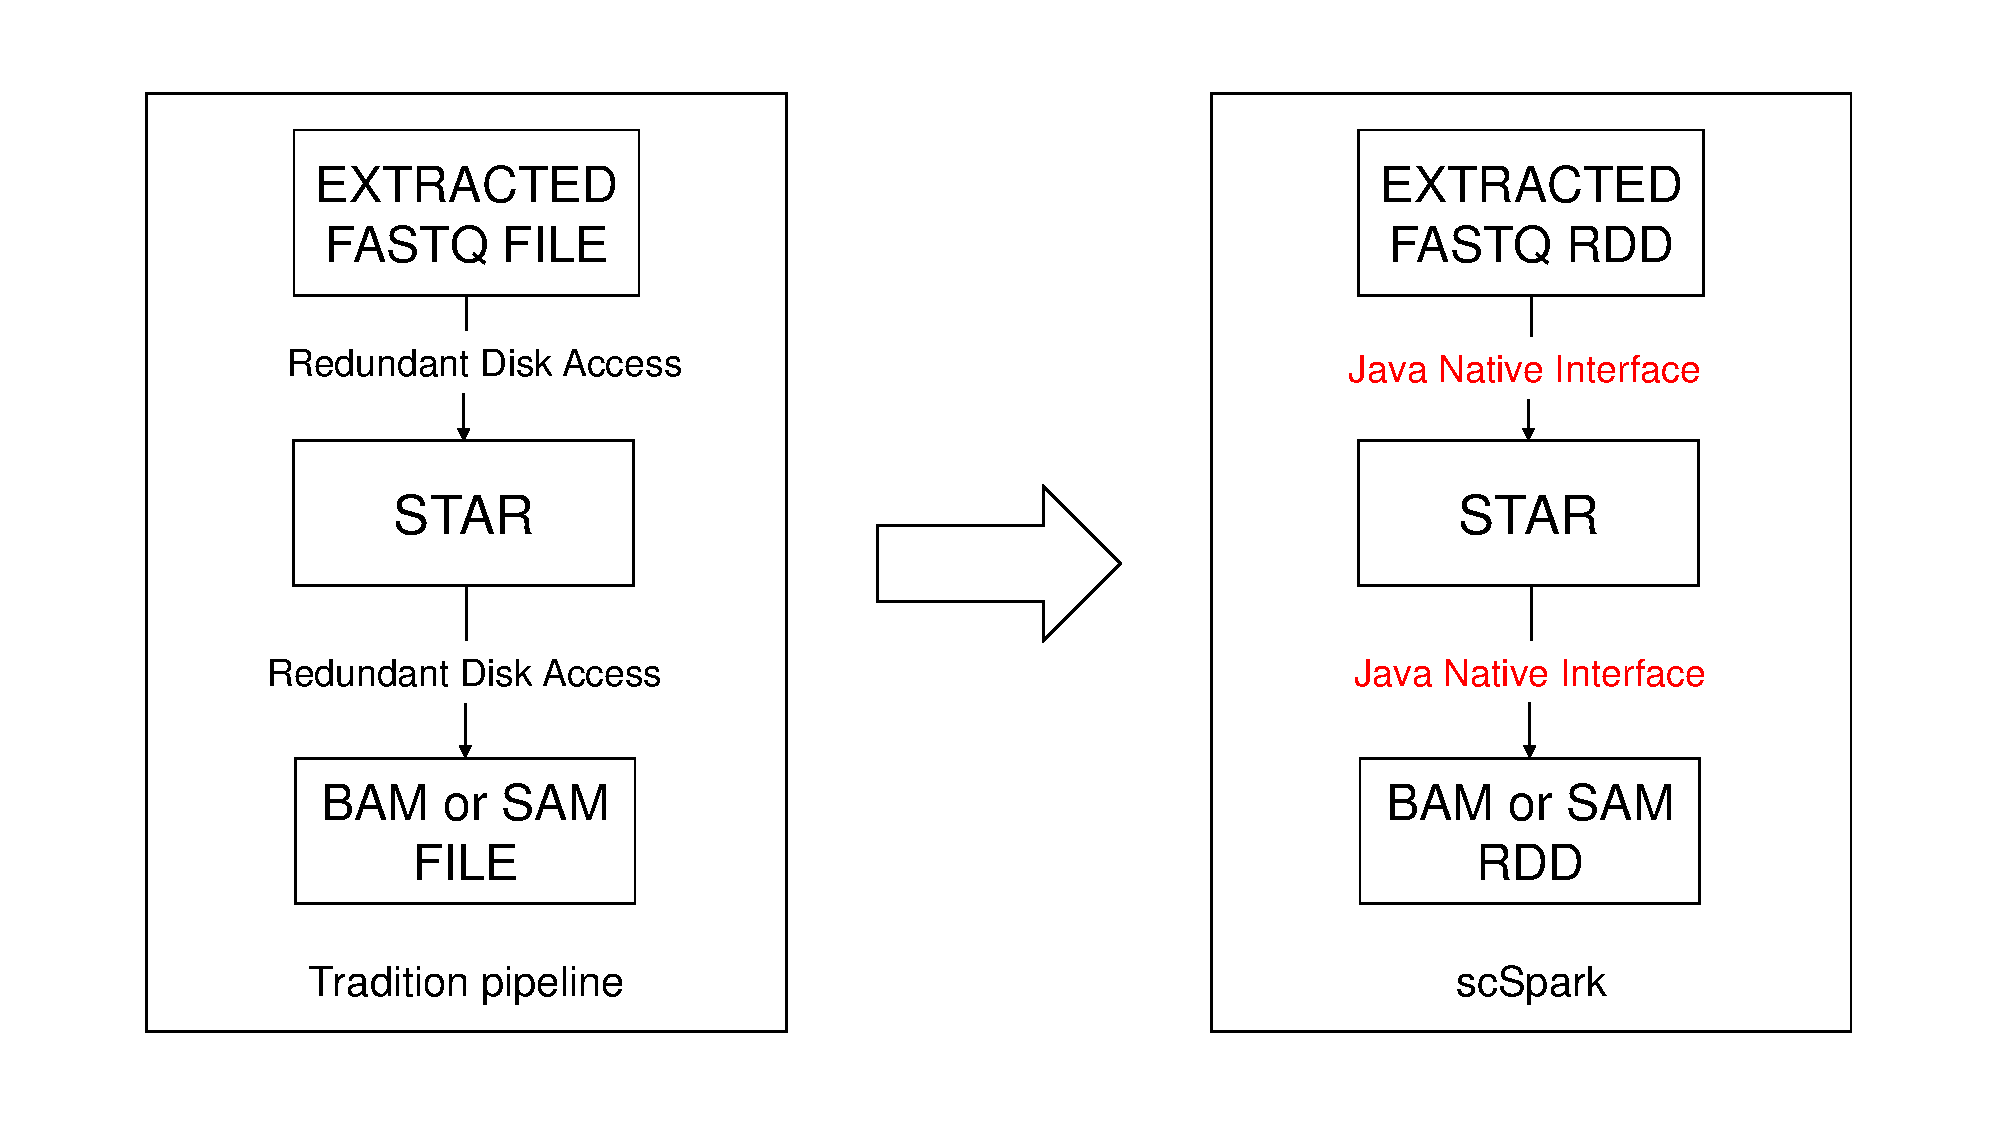
\includegraphics[width=\textwidth]{fig2.pdf}
  \caption{New way to implement STAR's interface.} \label{fig2}
\end{figure}
Apart from Cellranger we can't know how it implements because it isn't a open source software.
In tradition pipeline, STAR need load extracted FASTQ R2 file or load FASTQ R1 file, FASTQ R2 file and whitelist file that actually will generate unneccessary disk access.  
We choose STAR as our aligner but modify how STAR loads FASTQ file to avoid load extracted FASTQ R2 and FASTQ R1 twice. 
As shown in Fig~\ref{fig2}, we utilized Java Native Interface to transfer extracted FASTQ R2 RDD's data to STAR program, and then run the STAR process.
To overcome node's data volume imbalance problem, we repartition the extracted FASTQ R2 RDD, and then each node can run STAR parallel and with counterpoise data volume.
We also find if node's in memory is enough, we can start up more than one STAR's in one node to achieve better parallel.
STAR's result SAM or BAM file generate more disk access waste than STAR's input, we refer STAR-solo's solution to solve the problem by combining aligner and count.
We use Java Native Interface again to transfer STAR result and directly abstract them to SAM RDD.
This operation is parallel and totally in memory.

\subsection{Count with multi-node}
\begin{figure}
  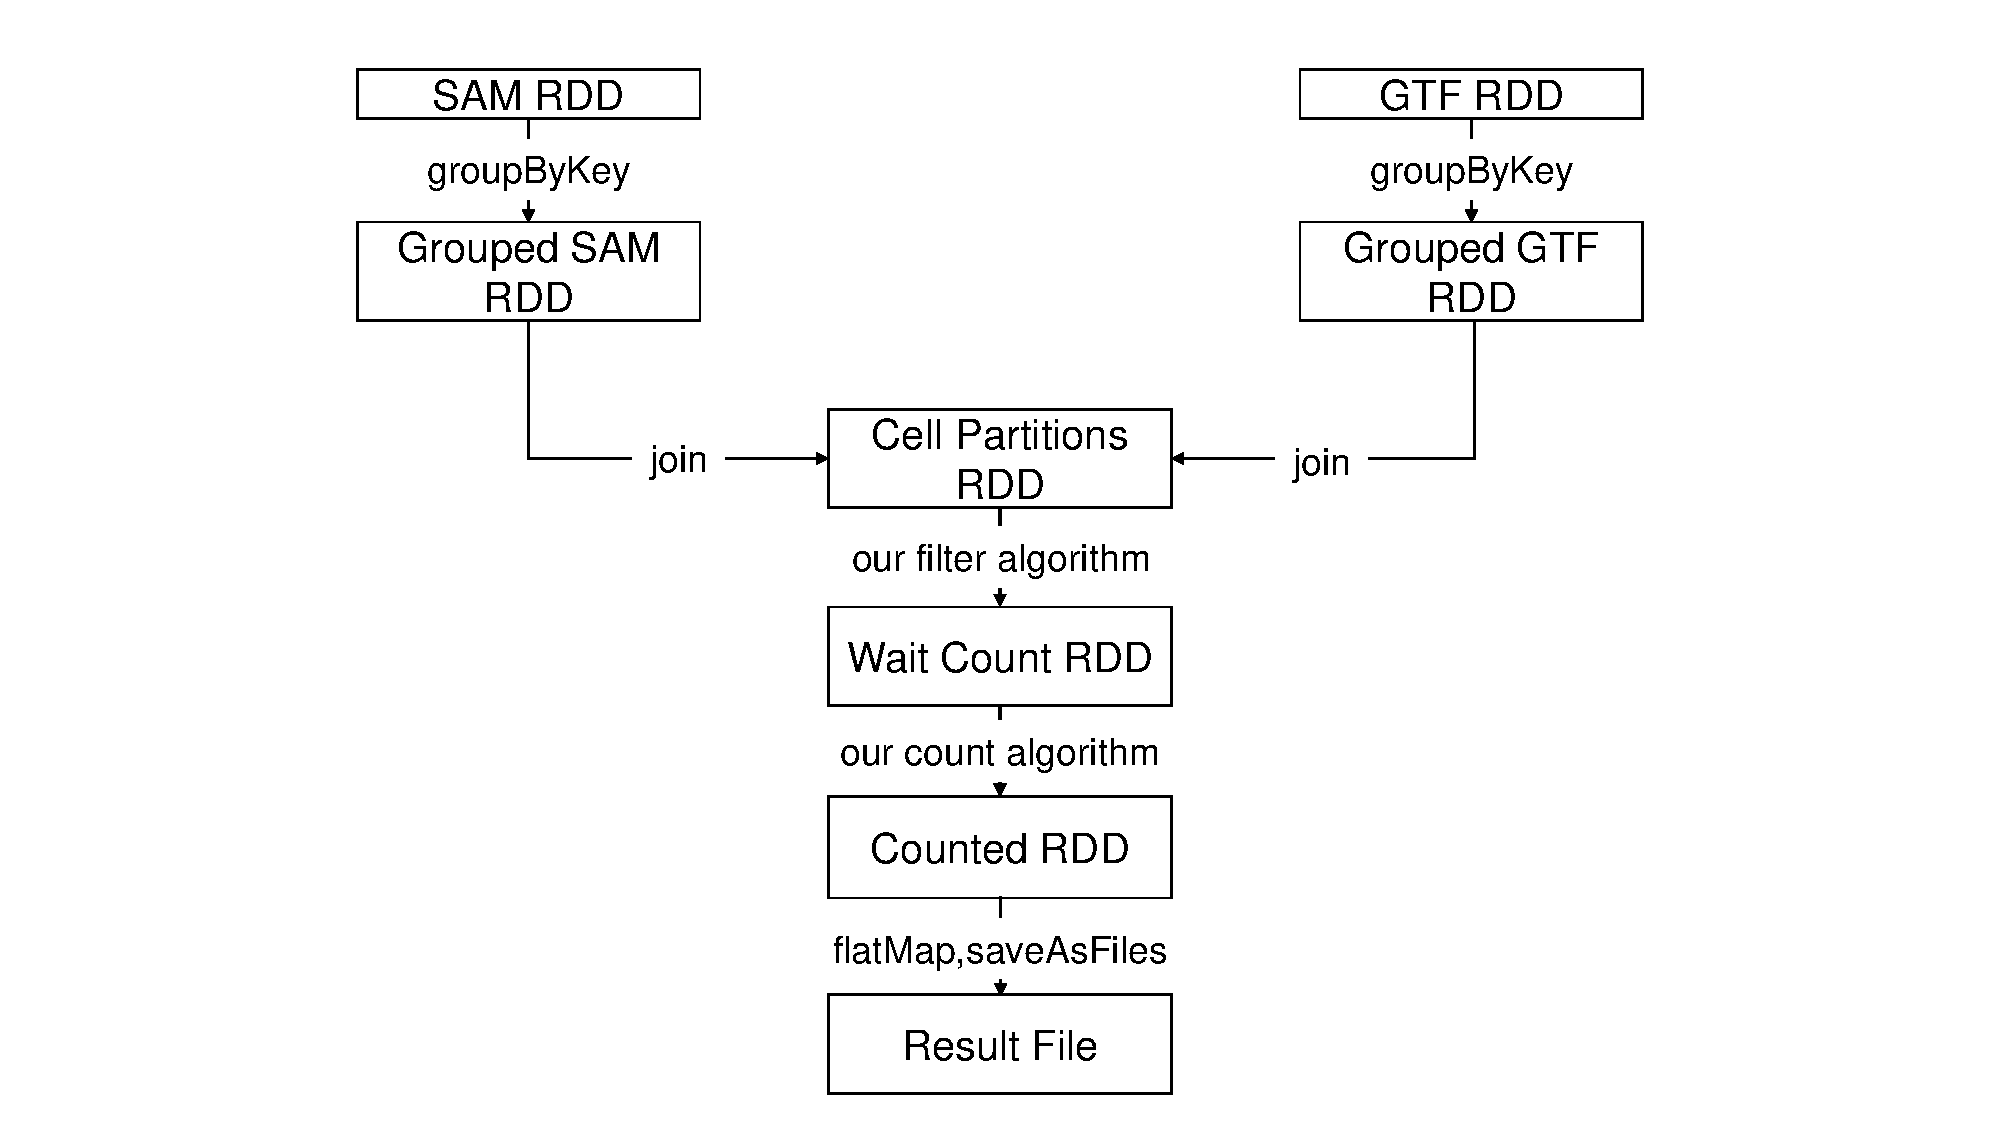
\includegraphics[width=\textwidth]{fig3.pdf}
  \caption{An overview of Spark version count.} \label{fig3}
\end{figure}
As shown in Fig~\ref{fig3}, to take advantage multi-node's compute capability, we used a new way to implement count step.
Except SAM RDD that generate in the previous step, we loaded GTF file to memory and abstract them as GTF RDD.
Then we grouped SAM RDD and GTF RDD by their cell name and due to different cell's record can't influence the other's count.
Then we used flatMap function to parallel compute each cell's read count.
In the end, we collected result in all nodes, and the result files will produce the only output disk access in the whole program.
ScSpark breaks the limitation of one node's compute and can scale easily.

\section{Results}
We evaluated the speed, scalabilty and compare each step's scalability of scSpark in this section.
First, we'll run our program and tradition pipeline and use process time to evaluated the advantage of scSpark.
And then, the index of speedup helps us to examify the scalability of scSpark.
In the end, we compared each step's scalability and found the reason why scSpark's scalability also has a ceiling.
\subsection{Experiment environments and Data Sets prepare}
We used Apache Spark version 2.1.0 as our in-memory computing environment.
The Spark cluster consists of Aliyun's ECS, and each node consists of 16 vCPU
(Intel Xeon(Cascade Lake) Platinum 8269CY at 2.5GHz), 128 GBytes of DRAM and 400 GBits ESSD.

An example scRNA-seq dataset generated by 10X Genomics on their platform was used in our experiments.
10X-PBMC-10k dataset: 10X Genomics v3 10k peripheral blood mononuclear cell (PBMC) from a healthy donor~\cite{ref_url4}. 
It contains two gzipped FASTQ files, after unzip, FASTQ R1's volume is 69 Gbytes, and FASTQ R2's volume is 144 Gbytes, each of that file contain 640 millions records.
We used STAR as our aligner, mapping to an index built on the human NCBI38 reference which called GRCh38.p12.genome.fa and use genome.gtf~\cite{ref_url5} to filter the SAM~\cite{ref_url5}.
To evaluate the reason of why scSpark have a scalability ceiling and to experiment more convenient, we split FASTQ file to 100 millions, 160 millions and 320 millions records,.
\subsection{Efficiency Evaluation}
\begin{table}
  \centering
  \caption{tradition pipelien and scSpark's performance compare}\label{tab1}
  \begin{tabular}{l | l | l  l}
  \hline
  System &  Cores & Spend time(s) \\
  \hline
   &  & 100 million(reads) & 640 million(reads) \\
  \hline
  UMI-tools & 64 cores & 7254 & 44160 \\
  \hline
  CellRanger & 64 cores & 6000 & 11700 \\
  \hline
  STAR-solo & 64 cores &  5820 & 8100 \\
  \hline
  scSpark & 4*16 cores & 354 & - \\
   & 8*16 cores & 210 & - \\
   & 16*16 cores & - & 841 \\
  \hline
  \end{tabular}
\end{table}
Limited by single machine's CPU cores, we only take 64 cores in traditional pipeline test as the traditional pipeline's performance.
Table~\ref{tab1} gives a summary of our program's performance and compare with tradition pipeline's performance.
We can see scSpark's speed is much more quick than any tradition pipeline in same CPU cores environment.
And scSpark can get improve when the cluster's CPU cores number increase.
\begin{table}
  \centering
  \caption{Each step performance compare}\label{tab2}
  \begin{tabular}{l | l | l | l | l}
  \hline
  System & Cores & filter & align & count \\
  \hline
  UMI-tools(100 million reads) & 64 cores & 9720 & 600 & 1740 \\
  \hline
  UMI-tools(640 million reads) & 64 cores & 33600 & 2160 & 8400 \\
  \hline
  scSpark(100 million reads) & 4*16 cores & 31 & 270 & 53 \\
  \hline
  scSpark(640 million reads) & 16*16 cores & 81 & 447 & 313 \\
  \hline
  \end{tabular}
\end{table}
Due to CellRanger isn't an open source software and STARsolo implements pipeline in a different way, we choose UMI-tools as scSpark each step's baseline.
As table~\ref{tab2} shown, scSpark is much faster than the traditional pipeline in any single step.
We can see the most significant improvement comes from the filter step because we make a traditional single thread operation to parallel computing in multi-machine and eliminate redundancy disk access.
For the same reason, scSpark's count step also gets considerable improvement.

\subsection{Scalability Evalution}
\begin{figure}
  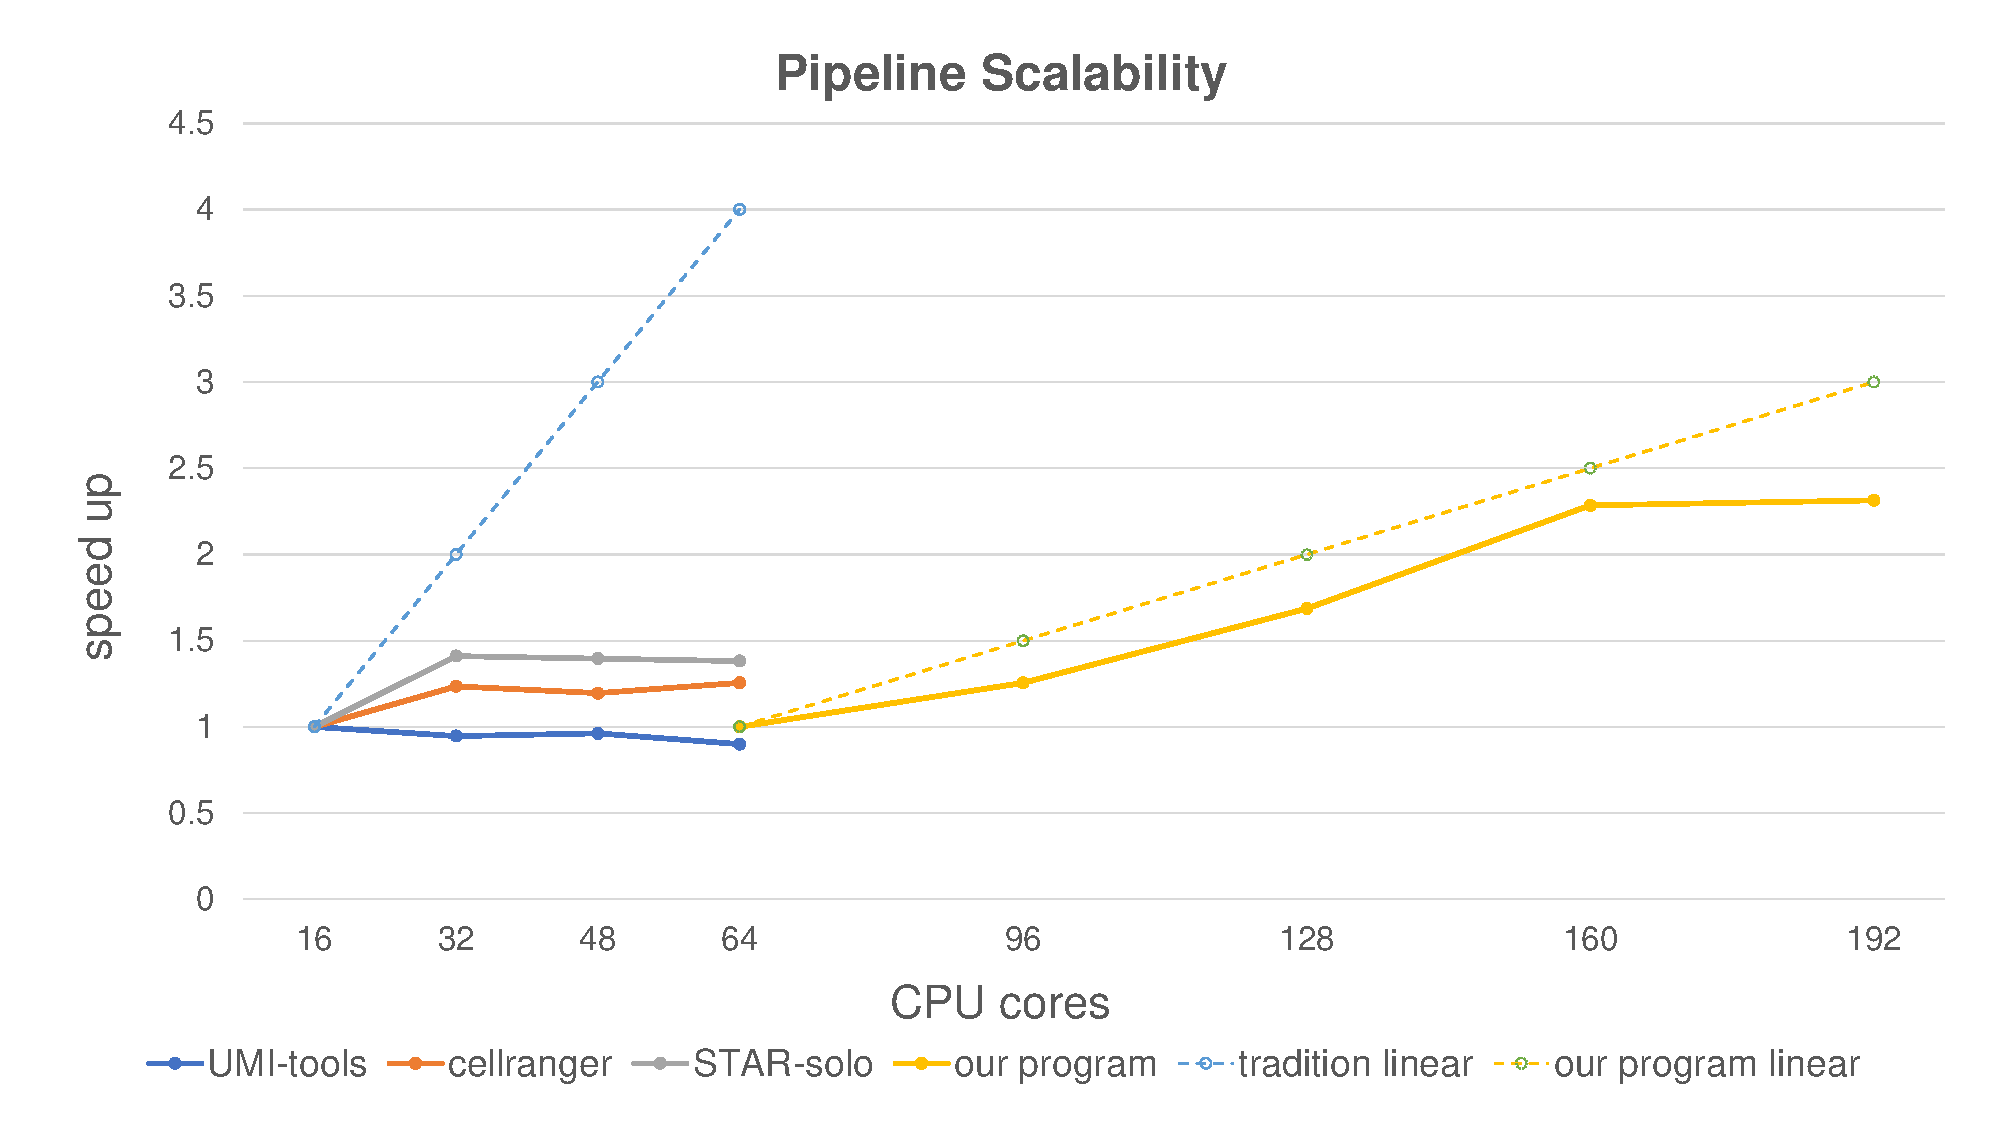
\includegraphics[width=\textwidth]{fig4.pdf}
  \caption{An overview of Spark version filter.} \label{fig4}
\end{figure}
ScSpark's second advantage is that it can get near linear improvement when the cluster's CPU core number improve.
To test the scalability of the tradition pipeline and scSpark, we use 16 CPU cores performance as tradition pipeline's baseline and 64 CPU cores performance as scSpark's baseline.
We use a small sample which have 100 millions records to compare speedup between our program and tradition pipeline.
As shown in Fig~\ref{fig5}, We found when CPU cores number increase our program can get near linear speedup and tradition pipeline's speedup far below linear speedup.
And we also found if the CPU cores number exceeds a ceiling, both tradition pipeline and scSpark will speedup nearly stop.
Umi-tools isn't showing any scalabiliy, even a little slow down when the CPU cores number increase.
STARsolo and CellRanger shows a little improve when the CPU cores increases to 32 from 16, but quickly stop speedup.
But scSpark ceiling is much higher than tradition pipeline.
All of it explain that our program more scalability than all tradition pipeline.
\subsection{Comparsion each step performance's increase}
\begin{figure}
  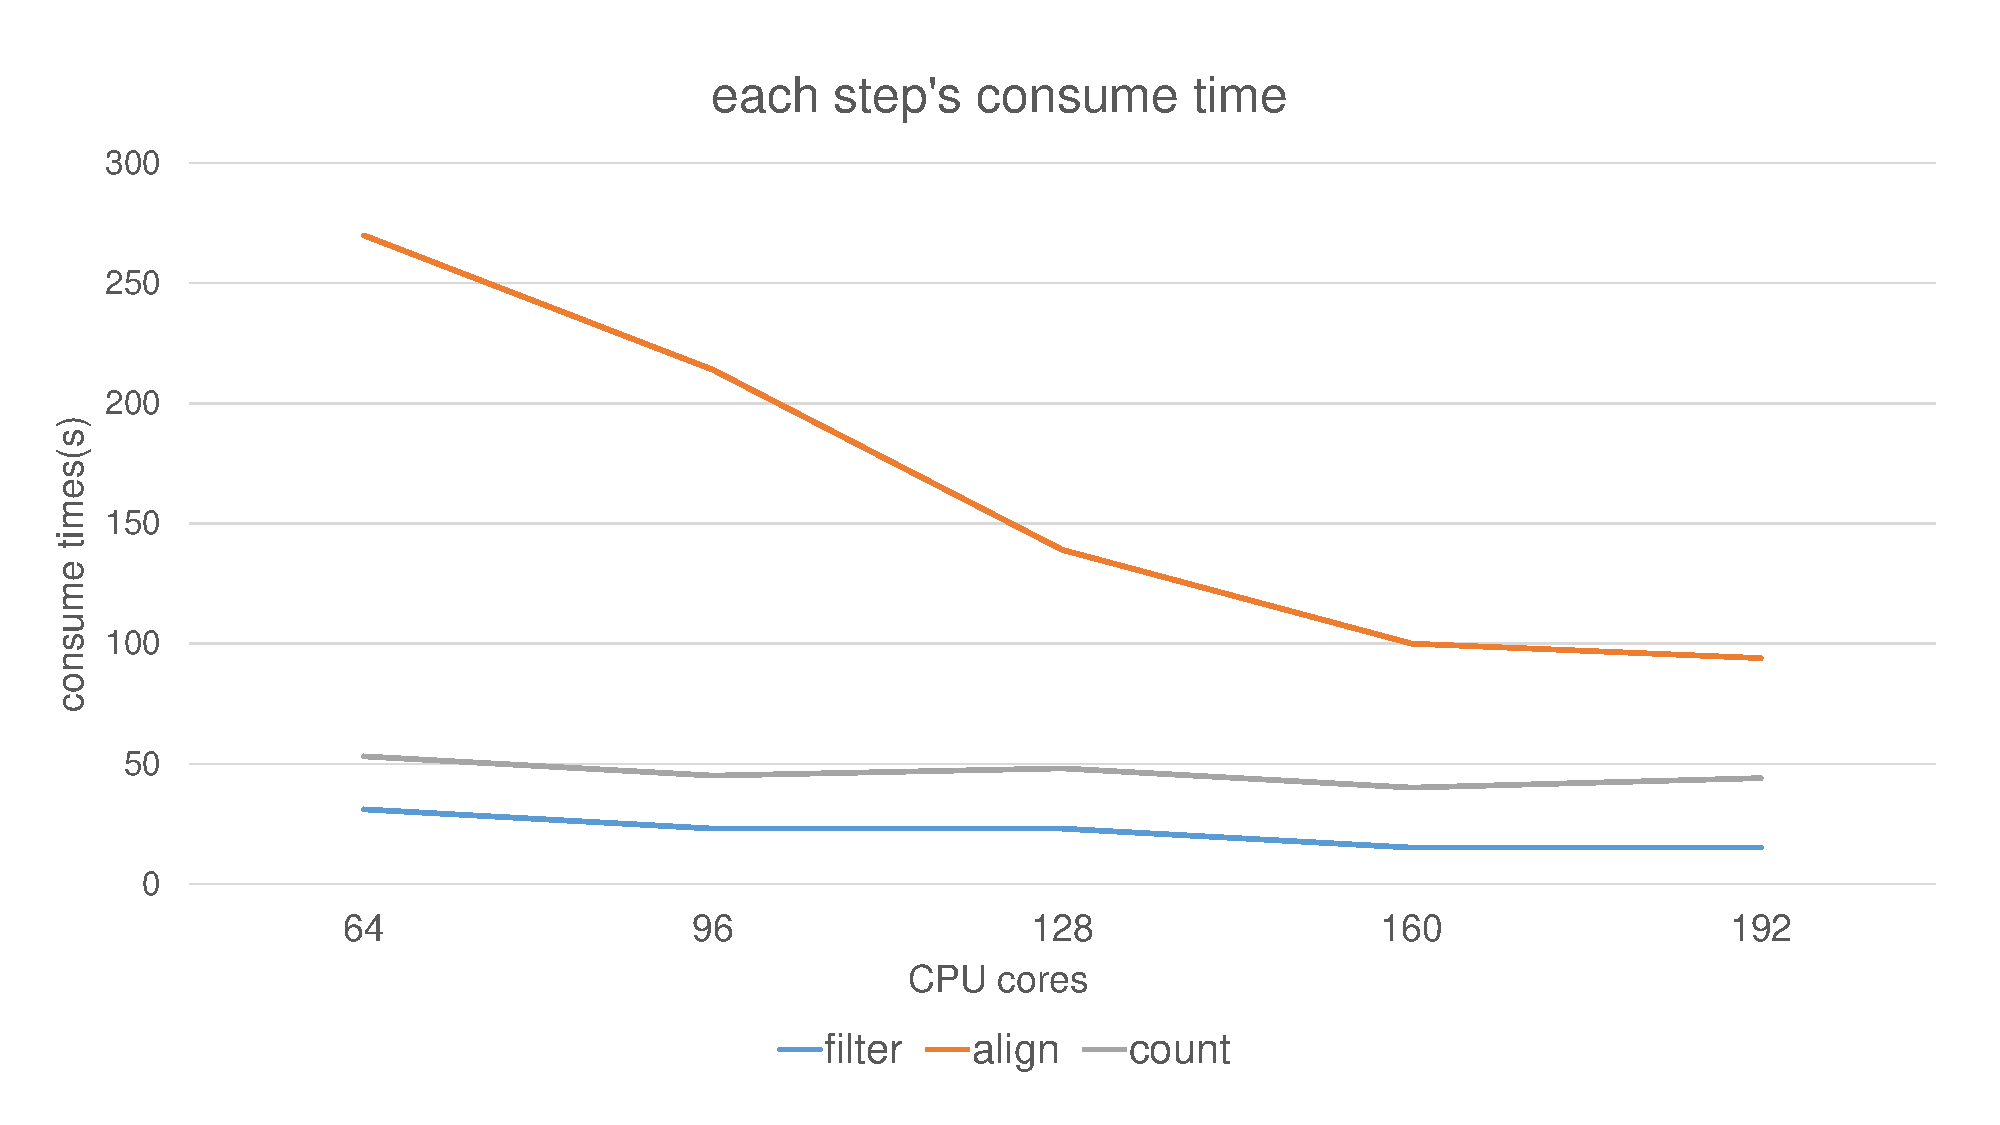
\includegraphics[width=\textwidth]{fig5.pdf}
  \caption{Each step consumes time.} \label{fig5}
\end{figure}
We also record each step's process time to know the reason of our improve and where can improve in future.
As shown in Fig~\ref{fig5}, we found our program's scalability most come from the align step and the align consumes most time in the whole program.
To find the reason why the align step is more scalability than the other step and why the scalability have a ceiling, we count how much records scSpark's STAR program can process.
We can find in Fig~\ref{fig6}, STAR's mapping speed is influenced by the data volume size and small volume dataset will lost its scalability earier than large volume dataset.
\begin{figure}
  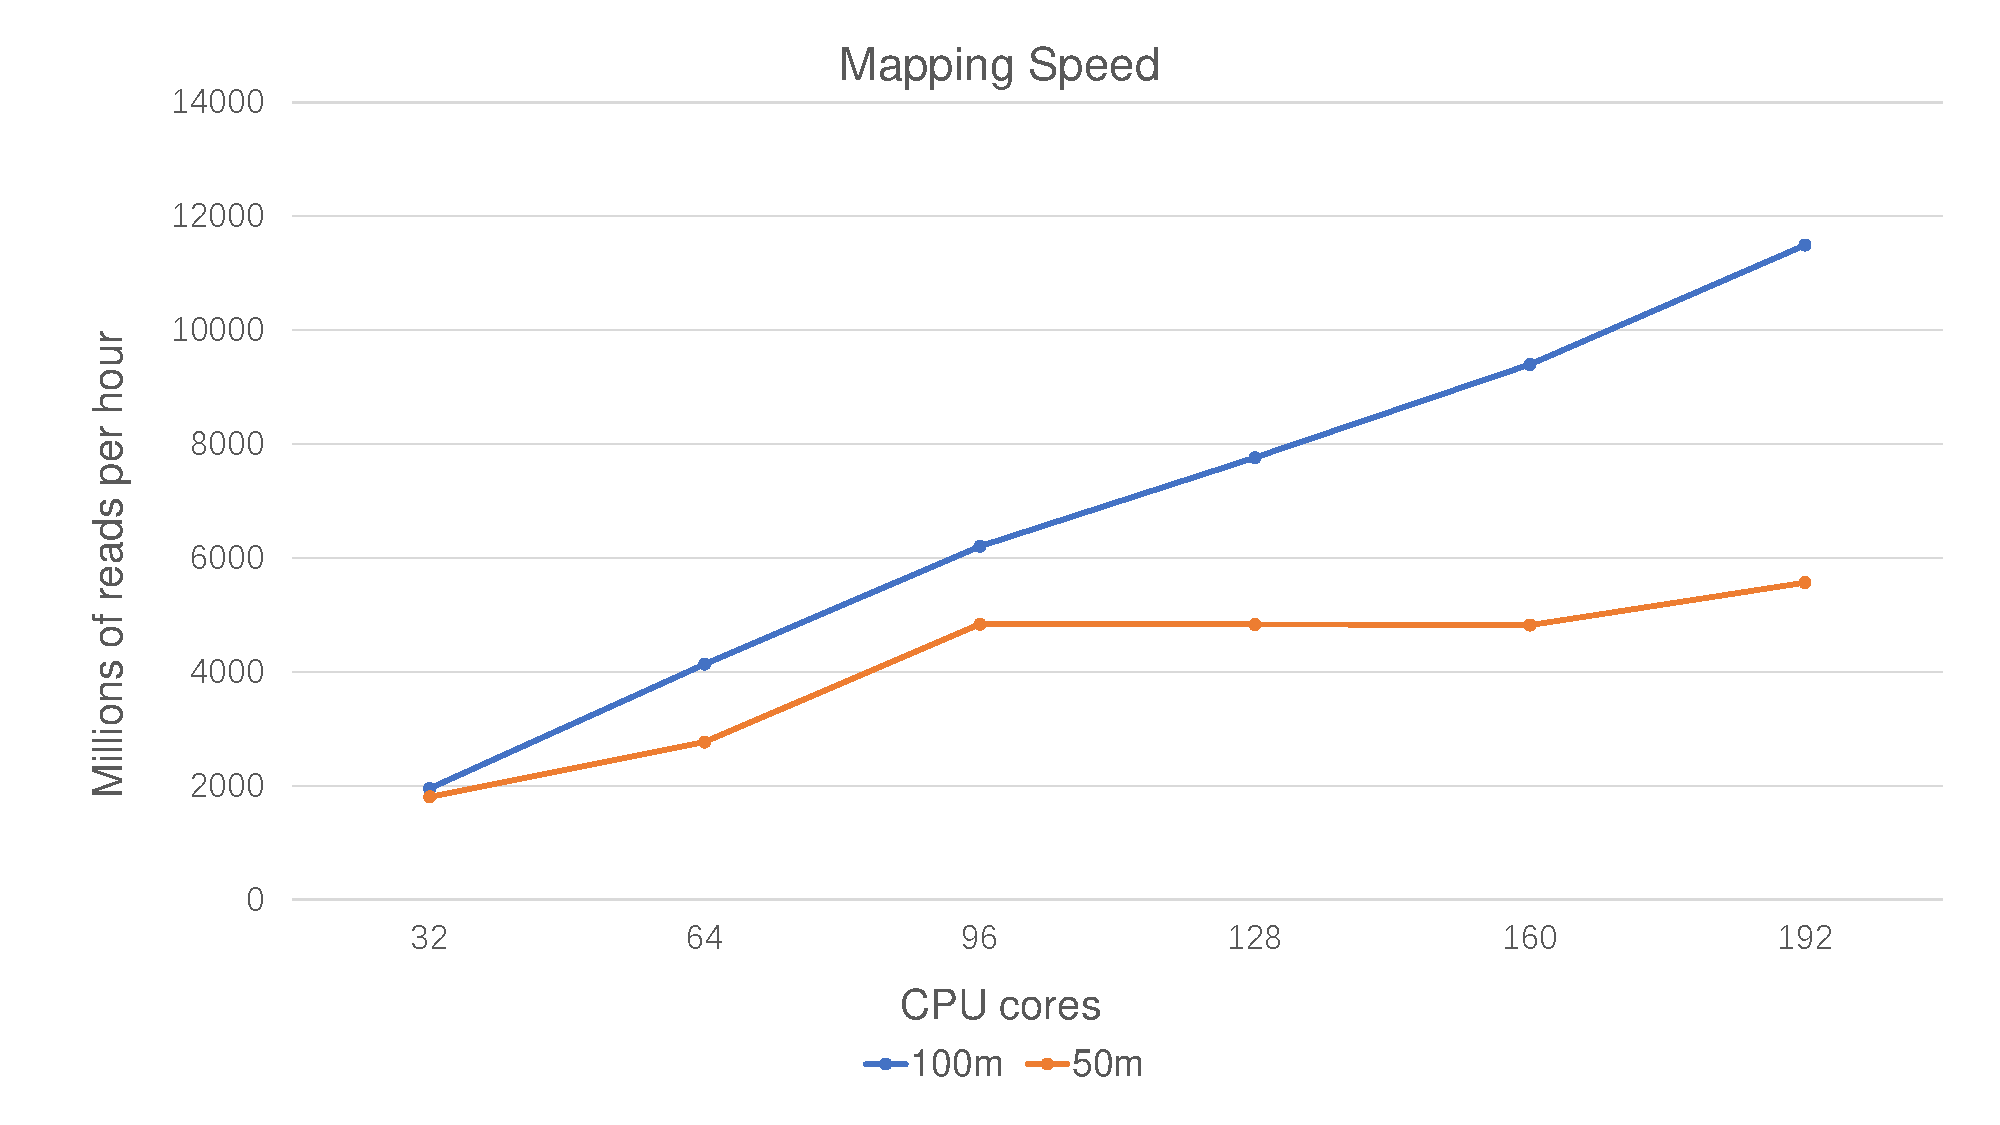
\includegraphics[width=\textwidth]{fig6.pdf}
  \caption{Invoked STAR's mapping step.} \label{fig6}
\end{figure}

\begin{table}
  \centering
  \caption{Data volume influence}\label{tab3}
  \begin{tabular}{l | l | l | l | l}
  \hline
  Data volume(Million reads) & 10 & 50 & 100 & 640 \\
  \hline
  mapping speed(Million of reads per hour) & 250.28 & 503.83 & 503.02 & 950 \\
  \hline
  \end{tabular}
\end{table}

Then we test STAR program, and find the mapping speed is influenced by data volume.
As Table~\ref{tab3} shown, STAR mapping speed will increase when the data volume increase.
So when we get scalability by increase partition, each partition's read number decrease will limit the scalability increase.

\subsection{Performance Analysis}
We tested performance to find bottleneck of our scSpark.
We used 640 millions records of FASTQ data to evaluate two aspect of our scSpark.
First we compared scSpark spend in network shuffle, disk access and compute time proportion to find whether network shuffle or disk access occupies too much time.
Second we tested CPU and memory usage, to ensure which resources will be scSpark's bottleneck.

\subsubsection{Network and Disk Behavior of scSpark}
\begin{figure}
  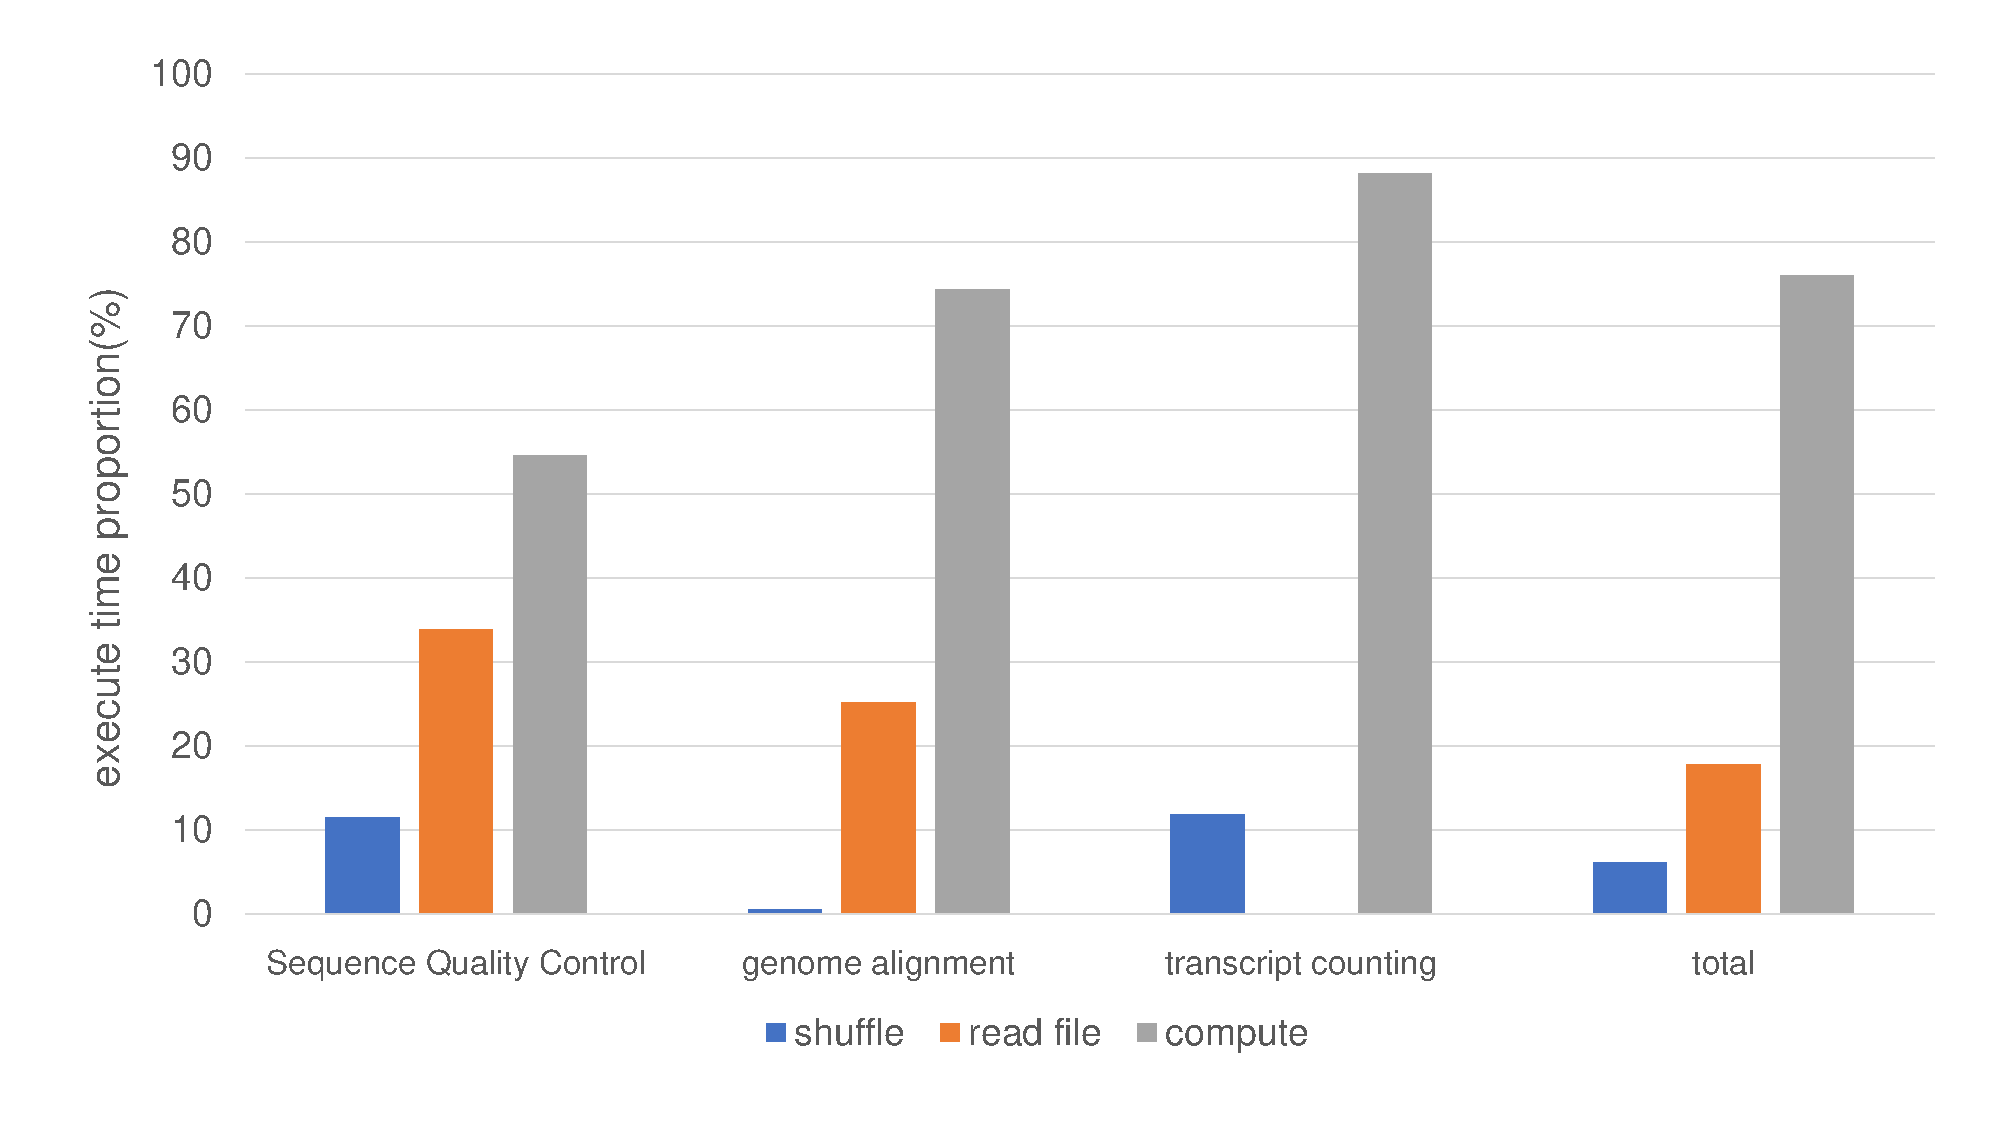
\includegraphics[width=\textwidth]{fig7.pdf}
  \caption{Each step consumes time.} \label{fig7}
\end{figure}
We computed network time by summing up the time that our scSpark shuffle data in multi machine.
Disk access comes from loading FASTQ, STAR's index and GTF files.
The ideal situation is tasks did not waste any time in disk access and network shuffle.
We found that scSpark's computing time occupies most execute time.
Except STAR's index file, all file's disk access distribute to each node that improve whole system's loading speed.
And we found the time that waste in shuffling doesn't occypy too much time.

\subsubsection{CPU and Memory usage of scSpark}
\begin{figure}
  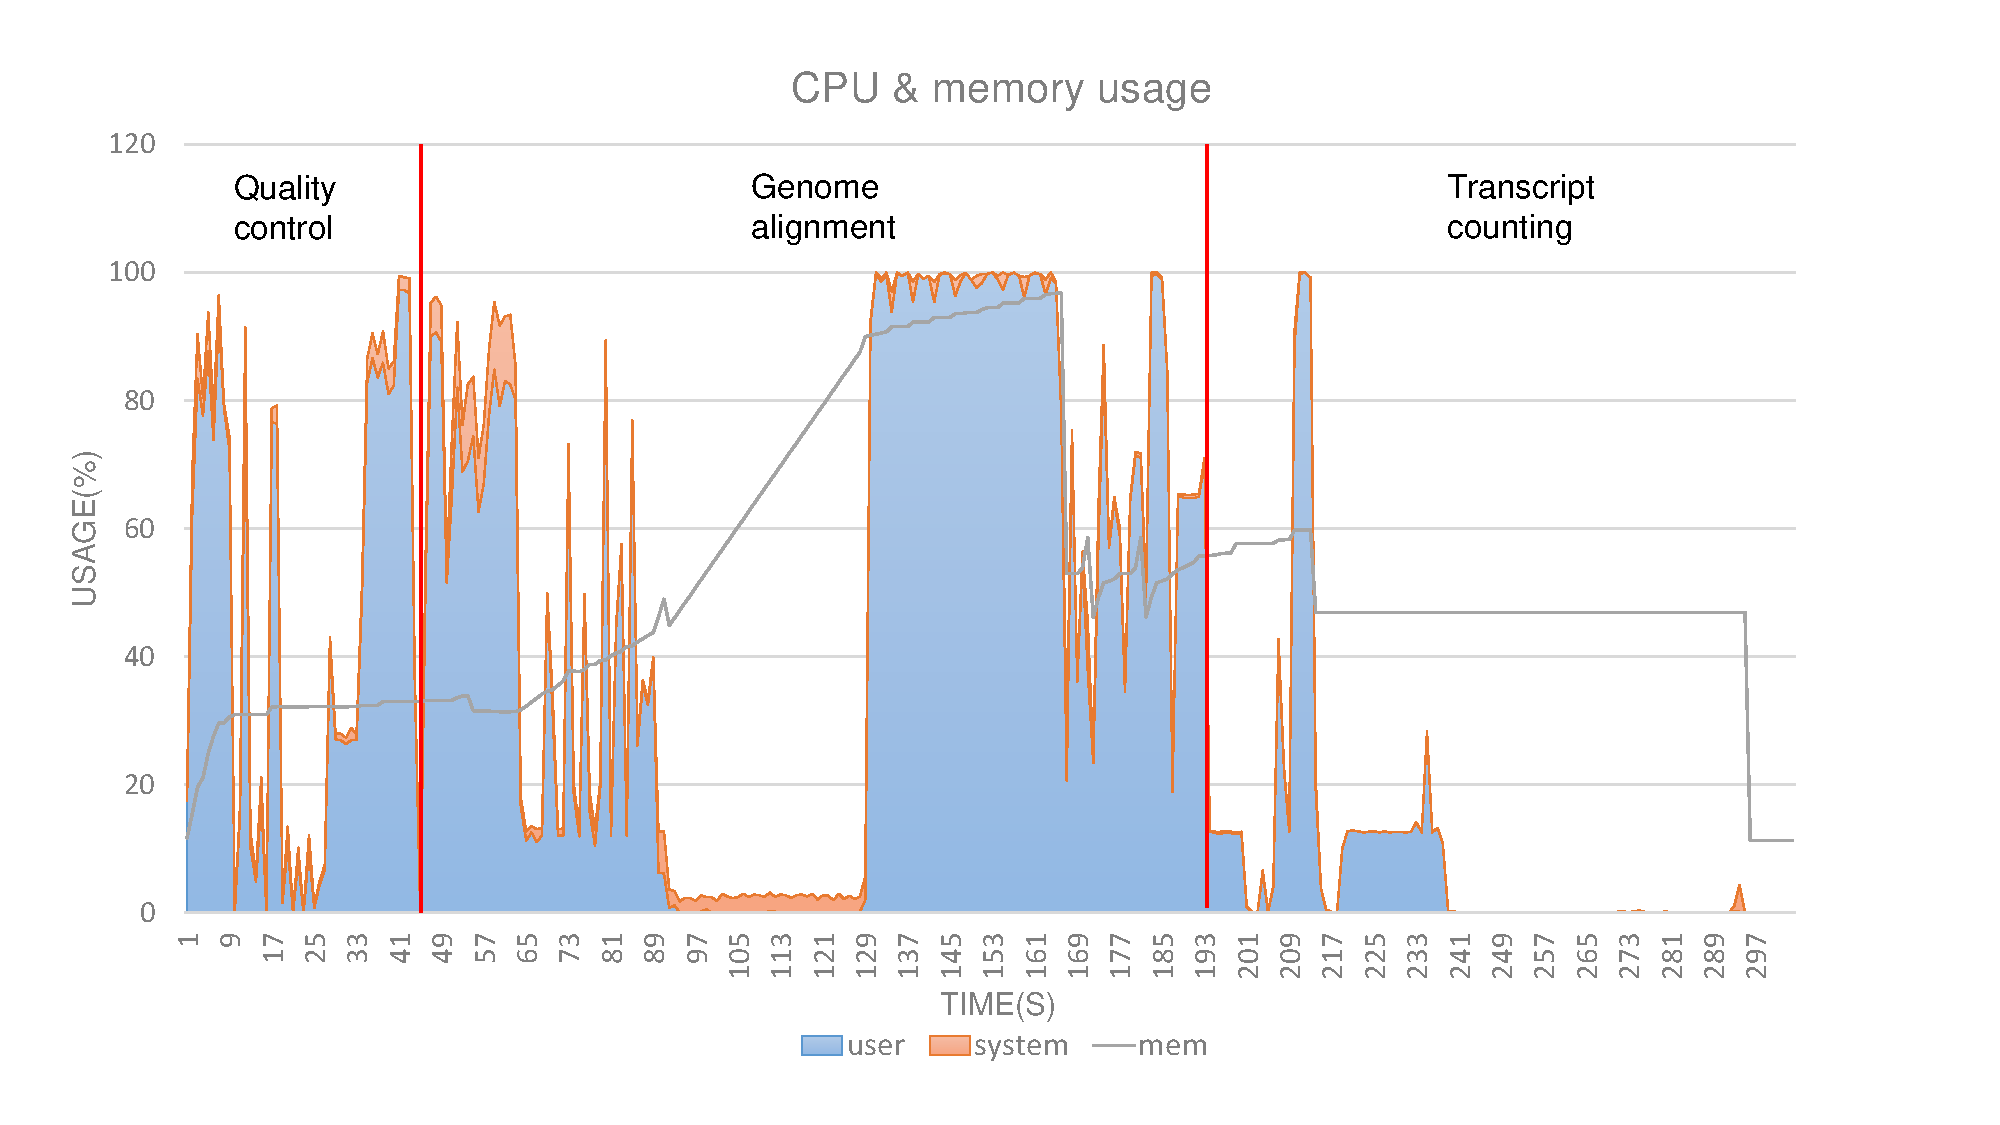
\includegraphics[width=\textwidth]{fig8.pdf}
  \caption{CPU and Memory usage of scSpark.} \label{fig8}
\end{figure}
We monitored scSpark's CPU and memory usage during processing.
As Fig~\ref{fig8} shown, in sequence quality control step, scSpark highly exploited each node's multi cores CPU to achieve speedup.
Convenition pipelines single thread solution's CPU usage is much lower than scSpark.
And we found that scSpark's boundary much comes from genome alignment.
Because we invoked STAR as our alignment tool, and STAR's program naturally occupy most proportion of memory in this step.

\subsubsection{Biological verification}
Our scSpark is developed based on UMI-tools.
And UMI-tools accuracy was fully verified.
This section we uses the gene expression matrix obtained by scSpark and UMI-tools under the same dataset to perform downstrema analysis of scRNA-seq data.
And then we compared two tools transcript analysis's result and cell cluster analysis's result to verify the correlation between scSpark and UMI-tools.
Under hgmm-1k-v3 dataset, we used scSpark and UMI-tools to get gene express matrix, compared two tools' result, and computed their correlation.
As Fig~\ref{fig9} shown, for each after processing cell barcode, their gene expression matrix approximate fit $y=x$, $R^{2}$ closed to 0.9998.
\begin{figure}
  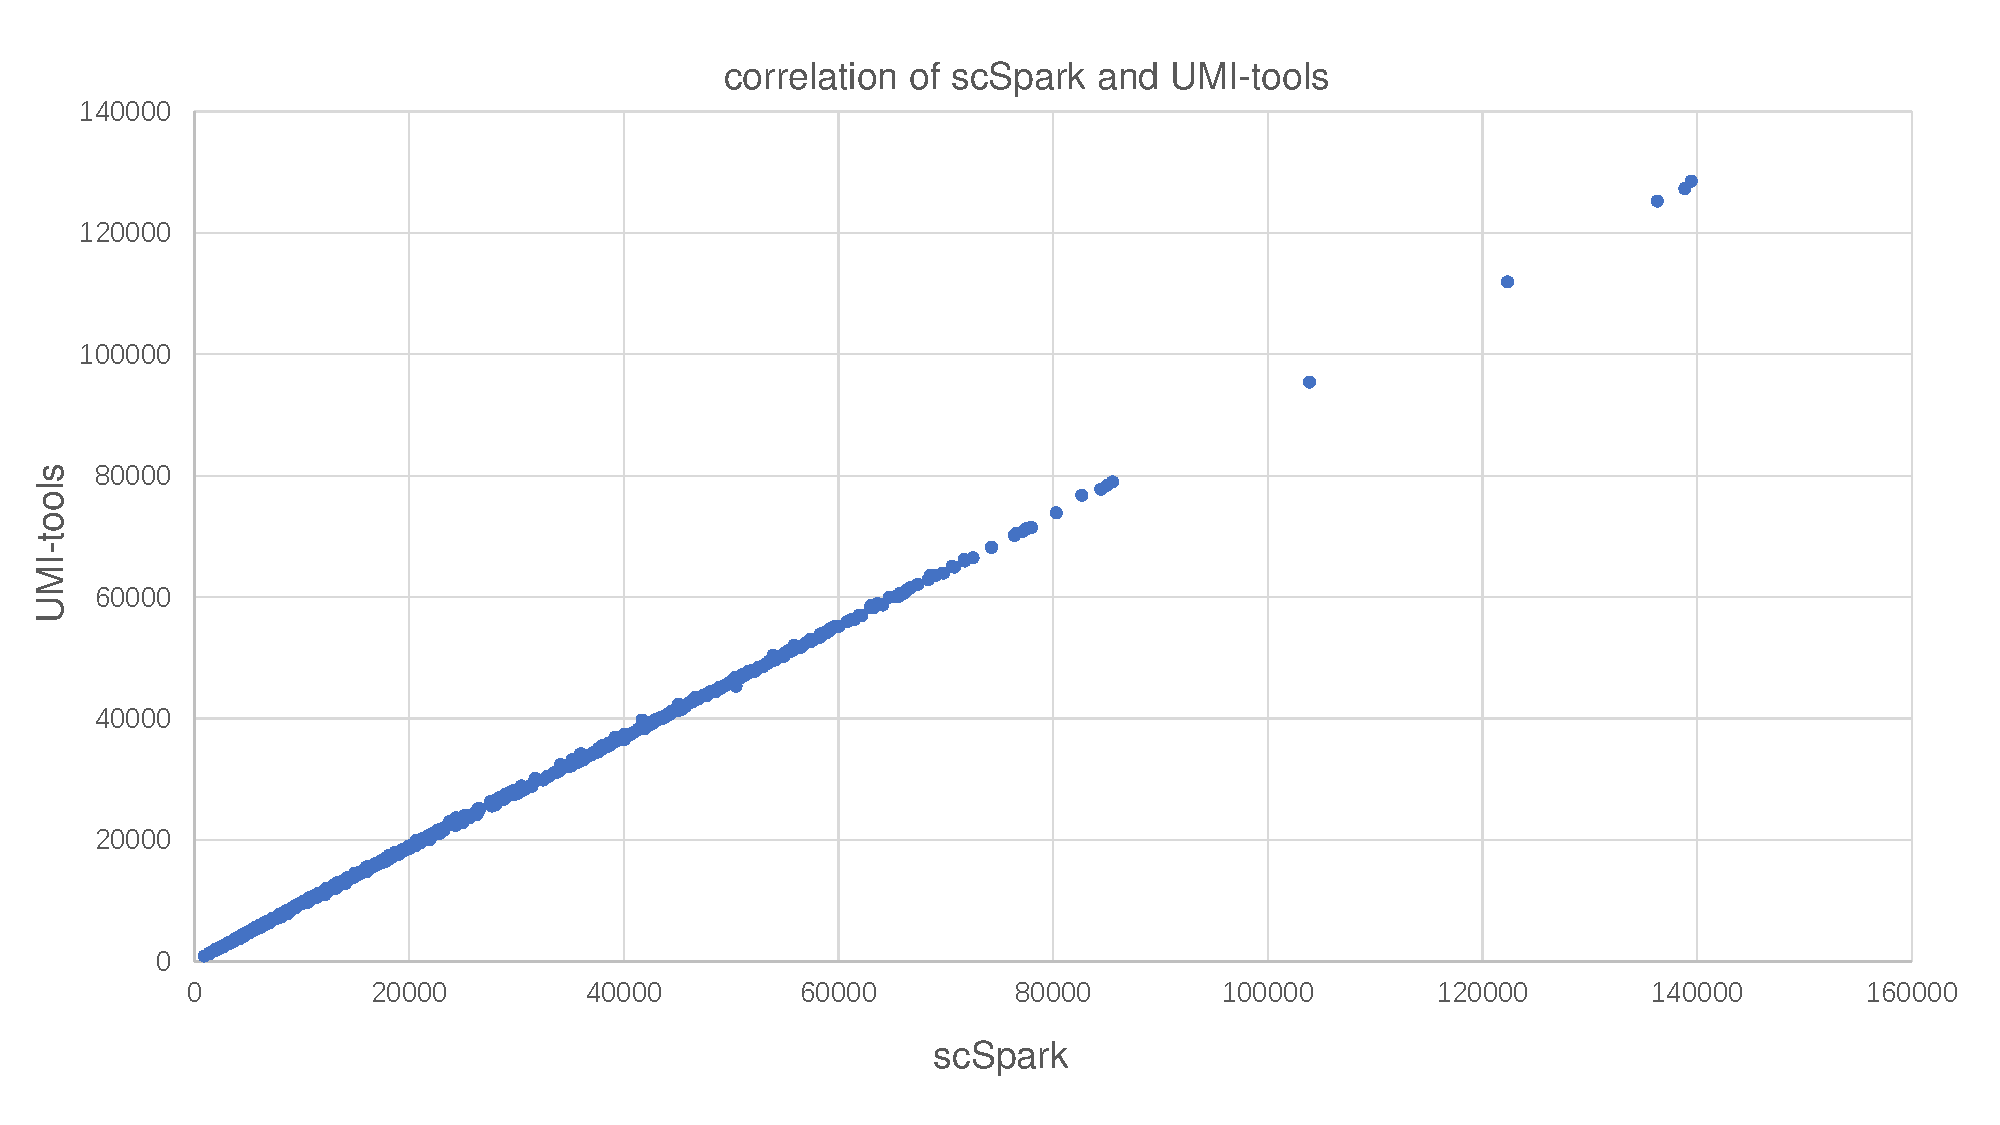
\includegraphics[width=\textwidth]{fig9.pdf}
  \caption{correlation of scSpark and UMI-tools.} \label{fig9}
\end{figure}
Furthermore, we used Seurat to print tSNE picture which based on gene expression matrix generated by ScSpark and UMI-tools.
And as Fig~\ref{fig10} shown, tSNE cell clustering result showed high corrleation between ScSpark and UMI-tools.
\begin{figure}
  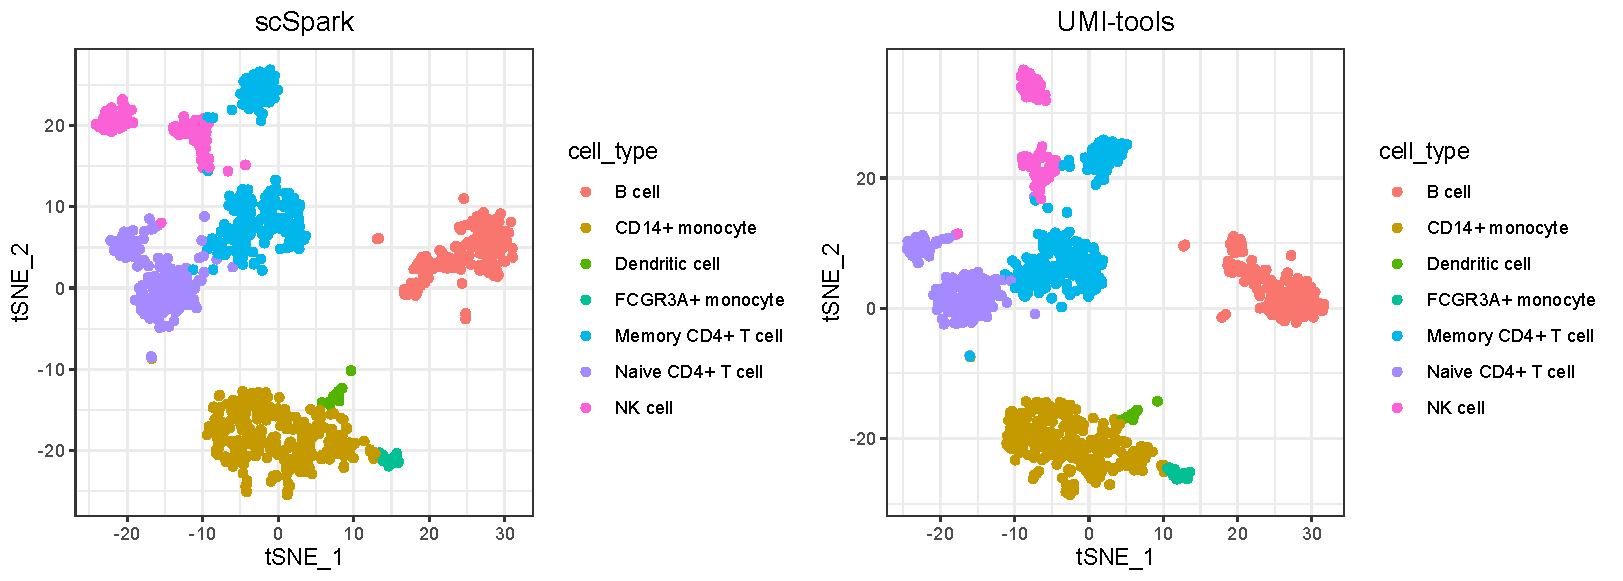
\includegraphics[width=\textwidth]{fig10.pdf}
  \caption{tSNE picture based on scSpark and UMI-tools' gene expression matrix.} \label{fig10}
\end{figure}
\section{Conclusion}
In this paper, we proposed a way which utilize Apache Spark's in memory compute trait and get considerable speedup and scalability.
Our scSpark can take advantage of multi machine compute capacity to speedup all step and eliminate redundant disk access.

Except performance improve, our scSpark also show much more scalability than any tradition pipeline which closes to linear improve.
Our scSpark not only can imporve each partition process STAR program's mapping speed, but also can improve scalabliity by increasing partition number if the resource is sufficient.

And we also found our scSpark's scalability improve has a ceiling.
The reason is that our scSpark invokes STAR's mapping speed influenced by loading index time.
And if data volume is tiny, the influence occupies a large proportion of whole the STAR program process time.

\begin{thebibliography}{8} 

\bibitem{Papalexi2018SinglecellRS}
Papalexi, E., Satija, R.: Single-cell rna sequencing to explore immune cell
heterogeneity. Nature Reviews Immunology  \textbf{18},  35--45 (2018)

\bibitem{Klein2015DropletBF}
Klein, A.M., Mazutis, L., Akartuna, I., Tallapragada, N., Veres, A., Li, V.,
Peshkin, L., Weitz, D., Kirschner, M.: Droplet barcoding for single-cell
transcriptomics applied to embryonic stem cells. Cell  \textbf{161},
1187--1201 (2015)
  
\bibitem{Macosko2015HighlyPG}
Macosko, E.Z., Basu, A., Satija, R., Nemesh, J., Shekhar, K., Goldman, M.,
Tirosh, I., Bialas, A., Kamitaki, N., Martersteck, E.M., Trombetta, J.J.,
Weitz, D., Sanes, J., Shalek, A., Regev, A., McCarroll, S.: Highly parallel
genome-wide expression profiling of individual cells using nanoliter
droplets. Cell  \textbf{161},  1202--1214 (2015)

\bibitem{tian2018scPipe}
Tian, L., Su, S., Dong, X., Amannzalcenstein, D., Biben, C., Seidi, A., Hilton,
D.J., Naik, S.H., Ritchie, M.E.: scpipe: A flexible r/bioconductor
preprocessing pipeline for single-cell rna-sequencing data. Plos One
\textbf{13}(7),  e0200193 (2018)

\bibitem{Kivioja2012Counting}
Kivioja, T., V?H?Rautio, A., Karlsson, K., Bonke, M., Enge, M., Linnarsson, S.,
Taipale, J.: Counting absolute numbers of molecules using unique molecular
identifiers. Nature Methods  \textbf{9}(1),  72--74 (2012)

\bibitem{camara2017Methods}
Camara, P.G.: Methods and challenges in the analysis of single-cell
rna-sequencing data. Current Opinion in Systems Biology  (2017)

\bibitem{dobin2012RNA}
Dobin, A., Davis, C.A., Schlesinger, F.: Rna-star : ultrafast universal spliced
sequences aligner : Supplementary materials. Hgdownload  (2012)

\bibitem{kim2015hisat}
Kim, D., Langmead, B., Salzberg, S.L.: Hisat: a fast spliced aligner with low
memory requirements. Nature methods  \textbf{12}(4),  357--360 (2015)

\bibitem{smith2017UMI}
Smith, T., Heger, A., Sudbery, I.: Umi-tools: modeling sequencing errors in
unique molecular identifiers to improve quantification accuracy. Genome
research  \textbf{27}(3), ~491 (2017)

\bibitem{swati0zUMIs}
Swati, P., Christoph, Z., Beate, V., Wolfgang, E., Ines, H.: zumis - a fast and
flexible pipeline to process rna sequencing data with umis. Gigaence (6), ~6

\bibitem{zheng2017Massively}
Zheng, G.X.Y., Terry, J.M., Belgrader, P., Ryvkin, P., Bent, Z.W., Wilson, R.,
Ziraldo, S.B., Wheeler, T.D., Mcdermott, G.P., Zhu, J.a.: Massively parallel
digital transcriptional profiling of single cells. Nature Communications
\textbf{8},  14049 (2017)

\bibitem{Svensson2017PowerAO}
Svensson, V., Natarajan, K., Ly, L.H., Miragaia, R., Labalette, C., Macaulay,
I., Cvejic, A., Teichmann, S.: Power analysis of single cell rna-sequencing
experiments. Nature methods  \textbf{14},  381 -- 387 (2017)

\bibitem{Petukhov2018dropEstPF}
Petukhov, V., Guo, J., Baryawno, N., Severe, N., Scadden, D., Samsonova, M.,
Kharchenko, P.: dropest: pipeline for accurate estimation of molecular counts
in droplet-based single-cell rna-seq experiments. Genome Biology  \textbf{19}
(2018)

\bibitem{Smith2017UMItoolsMS}
Smith, T., Heger, A., Sudbery, I.M.: Umi-tools: modeling sequencing errors in
unique molecular identifiers to improve quantification accuracy. Genome
research  \textbf{27 3},  491--499 (2017)

\bibitem{gao2020Comparison}
Gao, M., Ling, M., Tang, X., Wang, S., Xiao, X., Qiao, Y., Yang, W., Yu, R.:
Comparison of high-throughput single-cell rna sequencing data processing
pipelines  (02 2020). \doi{10.1101/2020.02.09.940221}

\bibitem{macosko2015Dropseq}
Macosko, E.Z., Basu, A., Satija, R., Nemesh, J., Shekhar, K., Goldman, M.,
Tirosh, I., Bialas, A.R., Kamitaki, N., Martersteck, E.M., Trombetta, J.J.,
Weitz, D.A., Sanes, J.R., Shalek, A.K., Regev, A., McCarroll, S.A.: Highly
parallel genome-wide expression profiling of individual cells using nanoliter
droplets. Cell  \textbf{161}(5),  1202—1214 (May 2015).
\doi{10.1016/j.cell.2015.05.002},
\url{https://europepmc.org/articles/PMC4481139}

\bibitem{macaulay0Svensson}
Svensson, V., Natarajan, K.N., Ly, L.H., Miragaia, R.J., Labalette, C.,
Macaulay, I.C., Cvejic, A., Teichmann, S.A.: Power analysis of single-cell
rna-sequencing experiments. Nature Methods

\bibitem{viktor2018dropEst}
Viktor, P., Jimin, G., Ninib, B., Nicolas, S., Scadden, D.T., Samsonova, M.G.,Kharchenko, P.V.: dropest: pipeline for accurate estimation of molecular
  counts in droplet-based single-cell rna-seq experiments. Genome Biology
\textbf{19}(1), ~78 (2018)

\bibitem{ref_url1}
UMI\_tools, \url{https://github.com/CGATOxford/UMI-tools}. Last accessed 30
Nov 2020

\bibitem{2019STARsolo}
Blibaum~A, W.J., A., D.: Starsolo: single-cell rna-seq analyses beyond gene
expression [version 1; not peer reviewed]. Genome Informatics  (2019)

\bibitem{ref_url2}
Apache Hadoop framework, \url{https://hadoop.apache.org}. Last accessed 30
Nov 2020

\bibitem{ref_url3}
Apache Spark framework, \url{https://spark.apache.org/}. Last accessed 30
Nov 2020

\bibitem{dean2008mapreduce}
Dean, J., Ghemawat, S.: Mapreduce: simplified data processing on large
clusters. Communications of the ACM  \textbf{51}(1),  107--113 (2008)

\bibitem{zaharia2012resilient}
Zaharia, M., Chowdhury, M., Das, T., Dave, A., Ma, J., McCauly, M., Franklin,
M.J., Shenker, S., Stoica, I.: Resilient distributed datasets: A
fault-tolerant abstraction for in-memory cluster computing. In: Presented as
part of the 9th $\{$USENIX$\}$ Symposium on Networked Systems Design and
Implementation ($\{$NSDI$\}$ 12). pp. 15--28 (2012)

\bibitem{abuin2016sparkbwa}
Abu{\'\i}n, J.M., Pichel, J.C., Pena, T.F., Amigo, J.: Sparkbwa: speeding up
the alignment of high-throughput dna sequencing data. PloS one
\textbf{11}(5),  e0155461 (2016)

\bibitem{li2018high}
Li, X., Tan, G., Wang, B., Sun, N.: High-performance genomic analysis framework
with in-memory computing. ACM SIGPLAN Notices  \textbf{53}(1),  317--328
(2018)

\bibitem{Yang2016Falco}
Yang, A., Michael, T., Lin, P., Ho, J.W.K.: Falco: a quick and flexible
single-cell rna-seq processing framework on the cloud. Bioinformatics (5), ~5
(2016)

\bibitem{ref_url4}
10xgenomics, \url{https://support.10xgenomics.com}. Last accessed 30
Nov 2020

\bibitem{ref_url5}
Index and GTF file, \url{https://www.gencodegenes.org/human/releases.html}. Last accessed 30
Nov 2020

\bibitem{divya2013elasticsearch}
Divya, M.S., Goyal, S.K.: Elasticsearch: An advanced and quick search technique
to handle voluminous data. Compusoft  \textbf{2}(6), ~171 (2013)

\bibitem{Baruzzo2017SimulationbasedCB}
Baruzzo, G., Hayer, K., Kim, E.J., Camillo, B.D., FitzGerald, G., Grant, G.:
  Simulation-based comprehensive benchmarking of rna-seq aligners. Nature
  Methods  \textbf{14},  135--139 (2017)

\bibitem{Cao2017ComprehensiveSC}
Cao, J., Packer, J.S., Ramani, V., Cusanovich, D.A., Huynh, C., Daza, R., Qiu,
  X., Lee, C., Furlan, S., Steemers, F., Adey, A.C., Waterston, R., Trapnell,
  C., Shendure, J.: Comprehensive single cell transcriptional profiling of a
  multicellular organism by combinatorial indexing. bioRxiv  (2017)

\bibitem{Klein2015DropletBF}
Klein, A.M., Mazutis, L., Akartuna, I., Tallapragada, N., Veres, A., Li, V.,
  Peshkin, L., Weitz, D., Kirschner, M.: Droplet barcoding for single-cell
  transcriptomics applied to embryonic stem cells. Cell  \textbf{161},
  1187--1201 (2015)

\bibitem{Macosko2015HighlyPG}
Macosko, E.Z., Basu, A., Satija, R., Nemesh, J., Shekhar, K., Goldman, M.,
  Tirosh, I., Bialas, A., Kamitaki, N., Martersteck, E.M., Trombetta, J.J.,
  Weitz, D., Sanes, J., Shalek, A., Regev, A., McCarroll, S.: Highly parallel
  genome-wide expression profiling of individual cells using nanoliter
  droplets. Cell  \textbf{161},  1202--1214 (2015)

\bibitem{Papalexi2018SinglecellRS}
Papalexi, E., Satija, R.: Single-cell rna sequencing to explore immune cell
  heterogeneity. Nature Reviews Immunology  \textbf{18},  35--45 (2018)

\bibitem{Rosenberg2018SinglecellPO}
Rosenberg, A., Roco, C.M., Muscat, R.A., Kuchina, A., Sample, P., Yao, Z.,
  Graybuck, L.T., Peeler, D.J., Mukherjee, S., Chen, W., Pun, S., Sellers,
  D.L., Tasic, B., Seelig, G.: Single-cell profiling of the developing mouse
  brain and spinal cord with split-pool barcoding. Science  \textbf{360},  176
  -- 182 (2018)

\bibitem{Smith2017UMItoolsMS}
Smith, T., Heger, A., Sudbery, I.M.: Umi-tools: modeling sequencing errors in
  unique molecular identifiers to improve quantification accuracy. Genome
  research  \textbf{27 3},  491--499 (2017)

\bibitem{Zhang2019ComparativeAO}
Zhang, X., Li, T., Liu, F., Chen, Y., Yao, J., Li, Z., Huang, Y., Wang, J.:
  Comparative analysis of droplet-based ultra-high-throughput single-cell
  rna-seq systems. Molecular cell  \textbf{73 1},  130--142.e5 (2019)

\bibitem{zheng2017Massivelypd}
Zheng, G.X.Y., Terry, J.M., Belgrader, P., Ryvkin, P., Bent, Z.W., Wilson, R.,
  Ziraldo, S.B., Wheeler, T.D., McDermott, G., Zhu, J., Gregory, M., Shuga, J.,
  Montesclaros, L., Underwood, J., Masquelier, D.A., Nishimura, S.Y.,
  Schnall-Levin, M., Wyatt, P.W., Hindson, C.M., Bharadwaj, R., Wong, A., Ness,
  K., Beppu, L., Deeg, H., McFarland, C., Loeb, K., Valente, W., Ericson, N.G.,
  Stevens, E., Radich, J., Mikkelsen, T., Hindson, B., Bielas, J.: Massively
  parallel digital transcriptional profiling of single cells. Nature
  Communications  \textbf{8} (2017)


\end{thebibliography}
\end{document}

